% Created by tikzDevice version 0.12.3 on 2019-12-11 20:53:32
% !TEX encoding = UTF-8 Unicode
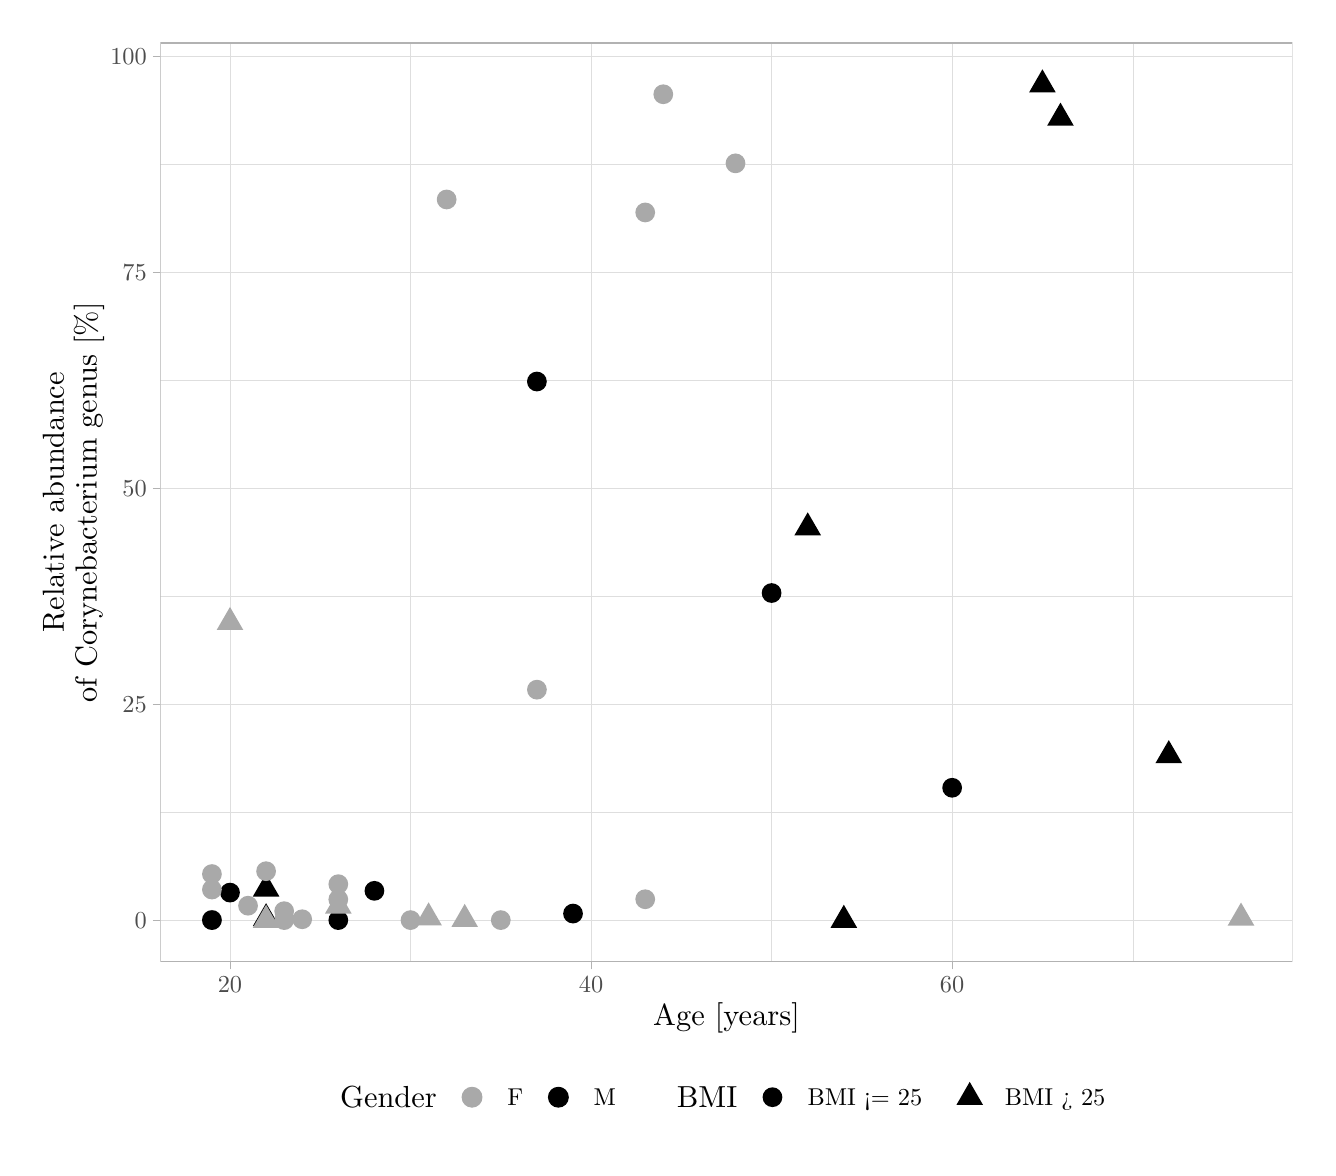
\begin{tikzpicture}[x=1pt,y=1pt]
\definecolor{fillColor}{RGB}{255,255,255}
\path[use as bounding box,fill=fillColor,fill opacity=0.00] (0,0) rectangle (462.53,404.71);
\begin{scope}
\path[clip] (  0.00,  0.00) rectangle (462.53,404.71);
\definecolor{drawColor}{RGB}{255,255,255}
\definecolor{fillColor}{RGB}{255,255,255}

\path[draw=drawColor,line width= 0.6pt,line join=round,line cap=round,fill=fillColor] (  0.00,  0.00) rectangle (462.53,404.71);
\end{scope}
\begin{scope}
\path[clip] ( 47.99, 67.14) rectangle (457.03,399.21);
\definecolor{fillColor}{RGB}{255,255,255}

\path[fill=fillColor] ( 47.99, 67.14) rectangle (457.03,399.21);
\definecolor{drawColor}{gray}{0.87}

\path[draw=drawColor,line width= 0.1pt,line join=round] ( 47.99,121.25) --
	(457.03,121.25);

\path[draw=drawColor,line width= 0.1pt,line join=round] ( 47.99,199.27) --
	(457.03,199.27);

\path[draw=drawColor,line width= 0.1pt,line join=round] ( 47.99,277.30) --
	(457.03,277.30);

\path[draw=drawColor,line width= 0.1pt,line join=round] ( 47.99,355.33) --
	(457.03,355.33);

\path[draw=drawColor,line width= 0.1pt,line join=round] (138.34, 67.14) --
	(138.34,399.21);

\path[draw=drawColor,line width= 0.1pt,line join=round] (268.82, 67.14) --
	(268.82,399.21);

\path[draw=drawColor,line width= 0.1pt,line join=round] (399.29, 67.14) --
	(399.29,399.21);

\path[draw=drawColor,line width= 0.3pt,line join=round] ( 47.99, 82.23) --
	(457.03, 82.23);

\path[draw=drawColor,line width= 0.3pt,line join=round] ( 47.99,160.26) --
	(457.03,160.26);

\path[draw=drawColor,line width= 0.3pt,line join=round] ( 47.99,238.29) --
	(457.03,238.29);

\path[draw=drawColor,line width= 0.3pt,line join=round] ( 47.99,316.31) --
	(457.03,316.31);

\path[draw=drawColor,line width= 0.3pt,line join=round] ( 47.99,394.34) --
	(457.03,394.34);

\path[draw=drawColor,line width= 0.3pt,line join=round] ( 73.11, 67.14) --
	( 73.11,399.21);

\path[draw=drawColor,line width= 0.3pt,line join=round] (203.58, 67.14) --
	(203.58,399.21);

\path[draw=drawColor,line width= 0.3pt,line join=round] (334.06, 67.14) --
	(334.06,399.21);
\definecolor{fillColor}{RGB}{169,169,169}

\path[fill=fillColor] (112.25, 89.68) circle (  3.57);

\path[fill=fillColor] (170.96, 82.23) circle (  3.57);

\path[fill=fillColor] ( 66.58, 98.87) circle (  3.57);

\path[fill=fillColor] (138.34, 82.23) circle (  3.57);

\path[fill=fillColor] (229.68,380.65) circle (  3.57);
\definecolor{fillColor}{RGB}{0,0,0}

\path[fill=fillColor] (112.25, 82.23) circle (  3.57);
\definecolor{fillColor}{RGB}{169,169,169}

\path[fill=fillColor] ( 73.11,195.39) --
	( 77.91,187.07) --
	( 68.30,187.07) --
	cycle;
\definecolor{fillColor}{RGB}{0,0,0}

\path[fill=fillColor] (197.06, 84.59) circle (  3.57);
\definecolor{fillColor}{RGB}{169,169,169}

\path[fill=fillColor] (223.15,337.93) circle (  3.57);
\definecolor{fillColor}{RGB}{0,0,0}

\path[fill=fillColor] (268.82,200.42) circle (  3.57);

\path[fill=fillColor] (294.91, 87.78) --
	(299.72, 79.46) --
	(290.11, 79.46) --
	cycle;
\definecolor{fillColor}{RGB}{169,169,169}

\path[fill=fillColor] (223.15, 89.77) circle (  3.57);
\definecolor{fillColor}{RGB}{0,0,0}

\path[fill=fillColor] (373.20,377.63) --
	(378.00,369.30) --
	(368.39,369.30) --
	cycle;
\definecolor{fillColor}{RGB}{169,169,169}

\path[fill=fillColor] (112.25, 92.92) --
	(117.06, 84.59) --
	(107.44, 84.59) --
	cycle;
\definecolor{fillColor}{RGB}{0,0,0}

\path[fill=fillColor] (412.34,147.27) --
	(417.15,138.95) --
	(407.53,138.95) --
	cycle;
\definecolor{fillColor}{RGB}{169,169,169}

\path[fill=fillColor] (184.01,165.50) circle (  3.57);

\path[fill=fillColor] ( 79.63, 87.43) circle (  3.57);
\definecolor{fillColor}{RGB}{0,0,0}

\path[fill=fillColor] ( 86.15, 99.06) --
	( 90.96, 90.74) --
	( 81.35, 90.74) --
	cycle;
\definecolor{fillColor}{RGB}{169,169,169}

\path[fill=fillColor] ( 99.20, 82.54) circle (  3.57);

\path[fill=fillColor] (112.25, 95.21) circle (  3.57);

\path[fill=fillColor] (157.92, 88.09) --
	(162.72, 79.76) --
	(153.11, 79.76) --
	cycle;
\definecolor{fillColor}{RGB}{0,0,0}

\path[fill=fillColor] (334.06,130.05) circle (  3.57);
\definecolor{fillColor}{RGB}{169,169,169}

\path[fill=fillColor] ( 86.15, 99.90) circle (  3.57);
\definecolor{fillColor}{RGB}{0,0,0}

\path[fill=fillColor] (281.87,229.59) --
	(286.67,221.27) --
	(277.06,221.27) --
	cycle;
\definecolor{fillColor}{RGB}{169,169,169}

\path[fill=fillColor] ( 66.58, 82.33) circle (  3.57);

\path[fill=fillColor] (255.77,355.68) circle (  3.57);
\definecolor{fillColor}{RGB}{0,0,0}

\path[fill=fillColor] ( 66.58, 82.23) circle (  3.57);
\definecolor{fillColor}{RGB}{169,169,169}

\path[fill=fillColor] (438.44, 88.58) --
	(443.24, 80.26) --
	(433.63, 80.26) --
	cycle;
\definecolor{fillColor}{RGB}{0,0,0}

\path[fill=fillColor] ( 86.15, 88.36) --
	( 90.96, 80.04) --
	( 81.35, 80.04) --
	cycle;

\path[fill=fillColor] (184.01,276.84) circle (  3.57);

\path[fill=fillColor] (366.67,389.67) --
	(371.48,381.34) --
	(361.87,381.34) --
	cycle;
\definecolor{fillColor}{RGB}{169,169,169}

\path[fill=fillColor] (151.39,342.63) circle (  3.57);

\path[fill=fillColor] ( 86.15, 87.78) --
	( 90.96, 79.46) --
	( 81.35, 79.46) --
	cycle;
\definecolor{fillColor}{RGB}{0,0,0}

\path[fill=fillColor] (125.30, 92.81) circle (  3.57);

\path[fill=fillColor] ( 73.11, 92.17) circle (  3.57);
\definecolor{fillColor}{RGB}{169,169,169}

\path[fill=fillColor] ( 92.68, 82.23) circle (  3.57);

\path[fill=fillColor] ( 92.68, 85.46) circle (  3.57);

\path[fill=fillColor] ( 66.58, 93.27) circle (  3.57);

\path[fill=fillColor] (144.87, 88.65) --
	(149.67, 80.32) --
	(140.06, 80.32) --
	cycle;
\definecolor{drawColor}{gray}{0.70}

\path[draw=drawColor,line width= 0.6pt,line join=round,line cap=round] ( 47.99, 67.14) rectangle (457.03,399.21);
\end{scope}
\begin{scope}
\path[clip] (  0.00,  0.00) rectangle (462.53,404.71);
\definecolor{drawColor}{gray}{0.30}

\node[text=drawColor,anchor=base east,inner sep=0pt, outer sep=0pt, scale=  0.88] at ( 43.04, 79.20) {0};

\node[text=drawColor,anchor=base east,inner sep=0pt, outer sep=0pt, scale=  0.88] at ( 43.04,157.23) {25};

\node[text=drawColor,anchor=base east,inner sep=0pt, outer sep=0pt, scale=  0.88] at ( 43.04,235.26) {50};

\node[text=drawColor,anchor=base east,inner sep=0pt, outer sep=0pt, scale=  0.88] at ( 43.04,313.28) {75};

\node[text=drawColor,anchor=base east,inner sep=0pt, outer sep=0pt, scale=  0.88] at ( 43.04,391.31) {100};
\end{scope}
\begin{scope}
\path[clip] (  0.00,  0.00) rectangle (462.53,404.71);
\definecolor{drawColor}{gray}{0.70}

\path[draw=drawColor,line width= 0.3pt,line join=round] ( 45.24, 82.23) --
	( 47.99, 82.23);

\path[draw=drawColor,line width= 0.3pt,line join=round] ( 45.24,160.26) --
	( 47.99,160.26);

\path[draw=drawColor,line width= 0.3pt,line join=round] ( 45.24,238.29) --
	( 47.99,238.29);

\path[draw=drawColor,line width= 0.3pt,line join=round] ( 45.24,316.31) --
	( 47.99,316.31);

\path[draw=drawColor,line width= 0.3pt,line join=round] ( 45.24,394.34) --
	( 47.99,394.34);
\end{scope}
\begin{scope}
\path[clip] (  0.00,  0.00) rectangle (462.53,404.71);
\definecolor{drawColor}{gray}{0.70}

\path[draw=drawColor,line width= 0.3pt,line join=round] ( 73.11, 64.39) --
	( 73.11, 67.14);

\path[draw=drawColor,line width= 0.3pt,line join=round] (203.58, 64.39) --
	(203.58, 67.14);

\path[draw=drawColor,line width= 0.3pt,line join=round] (334.06, 64.39) --
	(334.06, 67.14);
\end{scope}
\begin{scope}
\path[clip] (  0.00,  0.00) rectangle (462.53,404.71);
\definecolor{drawColor}{gray}{0.30}

\node[text=drawColor,anchor=base,inner sep=0pt, outer sep=0pt, scale=  0.88] at ( 73.11, 56.13) {20};

\node[text=drawColor,anchor=base,inner sep=0pt, outer sep=0pt, scale=  0.88] at (203.58, 56.13) {40};

\node[text=drawColor,anchor=base,inner sep=0pt, outer sep=0pt, scale=  0.88] at (334.06, 56.13) {60};
\end{scope}
\begin{scope}
\path[clip] (  0.00,  0.00) rectangle (462.53,404.71);
\definecolor{drawColor}{RGB}{0,0,0}

\node[text=drawColor,anchor=base,inner sep=0pt, outer sep=0pt, scale=  1.10] at (252.51, 44.09) {Age [years]};
\end{scope}
\begin{scope}
\path[clip] (  0.00,  0.00) rectangle (462.53,404.71);
\definecolor{drawColor}{RGB}{0,0,0}

\node[text=drawColor,rotate= 90.00,anchor=base,inner sep=0pt, outer sep=0pt, scale=  1.10] at ( 13.08,233.18) {Relative abundance };

\node[text=drawColor,rotate= 90.00,anchor=base,inner sep=0pt, outer sep=0pt, scale=  1.10] at ( 24.96,233.18) { of Corynebacterium genus [\%]};
\end{scope}
\begin{scope}
\path[clip] (  0.00,  0.00) rectangle (462.53,404.71);
\definecolor{fillColor}{RGB}{255,255,255}

\path[fill=fillColor] (107.41,  5.50) rectangle (218.06, 30.95);
\end{scope}
\begin{scope}
\path[clip] (  0.00,  0.00) rectangle (462.53,404.71);
\definecolor{drawColor}{RGB}{0,0,0}

\node[text=drawColor,anchor=base west,inner sep=0pt, outer sep=0pt, scale=  1.10] at (112.91, 14.44) {Gender};
\end{scope}
\begin{scope}
\path[clip] (  0.00,  0.00) rectangle (462.53,404.71);
\definecolor{fillColor}{RGB}{255,255,255}

\path[fill=fillColor] (153.34, 11.00) rectangle (167.80, 25.45);
\end{scope}
\begin{scope}
\path[clip] (  0.00,  0.00) rectangle (462.53,404.71);
\definecolor{drawColor}{RGB}{169,169,169}
\definecolor{fillColor}{RGB}{169,169,169}

\path[draw=drawColor,line width= 0.4pt,line join=round,line cap=round,fill=fillColor] (160.57, 18.23) circle (  3.57);
\end{scope}
\begin{scope}
\path[clip] (  0.00,  0.00) rectangle (462.53,404.71);
\definecolor{fillColor}{RGB}{255,255,255}

\path[fill=fillColor] (184.54, 11.00) rectangle (198.99, 25.45);
\end{scope}
\begin{scope}
\path[clip] (  0.00,  0.00) rectangle (462.53,404.71);
\definecolor{drawColor}{RGB}{0,0,0}
\definecolor{fillColor}{RGB}{0,0,0}

\path[draw=drawColor,line width= 0.4pt,line join=round,line cap=round,fill=fillColor] (191.77, 18.23) circle (  3.57);
\end{scope}
\begin{scope}
\path[clip] (  0.00,  0.00) rectangle (462.53,404.71);
\definecolor{drawColor}{RGB}{0,0,0}

\node[text=drawColor,anchor=base west,inner sep=0pt, outer sep=0pt, scale=  0.88] at (173.30, 15.20) {F};
\end{scope}
\begin{scope}
\path[clip] (  0.00,  0.00) rectangle (462.53,404.71);
\definecolor{drawColor}{RGB}{0,0,0}

\node[text=drawColor,anchor=base west,inner sep=0pt, outer sep=0pt, scale=  0.88] at (204.49, 15.20) {M};
\end{scope}
\begin{scope}
\path[clip] (  0.00,  0.00) rectangle (462.53,404.71);
\definecolor{fillColor}{RGB}{255,255,255}

\path[fill=fillColor] (229.06,  5.50) rectangle (397.61, 30.95);
\end{scope}
\begin{scope}
\path[clip] (  0.00,  0.00) rectangle (462.53,404.71);
\definecolor{drawColor}{RGB}{0,0,0}

\node[text=drawColor,anchor=base west,inner sep=0pt, outer sep=0pt, scale=  1.10] at (234.56, 14.44) {BMI};
\end{scope}
\begin{scope}
\path[clip] (  0.00,  0.00) rectangle (462.53,404.71);
\definecolor{fillColor}{RGB}{255,255,255}

\path[fill=fillColor] (261.90, 11.00) rectangle (276.35, 25.45);
\end{scope}
\begin{scope}
\path[clip] (  0.00,  0.00) rectangle (462.53,404.71);
\definecolor{fillColor}{RGB}{0,0,0}

\path[fill=fillColor] (269.13, 18.23) circle (  3.57);
\end{scope}
\begin{scope}
\path[clip] (  0.00,  0.00) rectangle (462.53,404.71);
\definecolor{fillColor}{RGB}{255,255,255}

\path[fill=fillColor] (333.18, 11.00) rectangle (347.63, 25.45);
\end{scope}
\begin{scope}
\path[clip] (  0.00,  0.00) rectangle (462.53,404.71);
\definecolor{fillColor}{RGB}{0,0,0}

\path[fill=fillColor] (340.40, 23.78) --
	(345.21, 15.45) --
	(335.60, 15.45) --
	cycle;
\end{scope}
\begin{scope}
\path[clip] (  0.00,  0.00) rectangle (462.53,404.71);
\definecolor{drawColor}{RGB}{0,0,0}

\node[text=drawColor,anchor=base west,inner sep=0pt, outer sep=0pt, scale=  0.88] at (281.85, 15.20) {BMI <= 25};
\end{scope}
\begin{scope}
\path[clip] (  0.00,  0.00) rectangle (462.53,404.71);
\definecolor{drawColor}{RGB}{0,0,0}

\node[text=drawColor,anchor=base west,inner sep=0pt, outer sep=0pt, scale=  0.88] at (353.13, 15.20) {BMI > 25};
\end{scope}
\end{tikzpicture}
